\chapter{Modelling The Energy Usage And Carbon Emissions Of Ethereum}
\label{Modelling}

% ____________________________________________________________________________
\section{Chapter Summary}


% ____________________________________________________________________________

% %  MODEL AAAAAAAAAAAAAAAAAAAAAAAAAAAAAAAAAAAAAAAAAA
% \subsection{Model A}
% From the research,it seems like power usage is usually not the limiting factor but rather the storage space needed to run validators.

% The recommended hardware for a validator one is shown in table \_\_ of the appendix as well as in the table below. \_\_

% So according to this hardware recommendation, we could estimate the power usage depending on statistics provided by manufacturers. Let's assume the same configuration of hardware as in the \cite{CryptoCarbonRatingsInstitute2022TheNetwork} (They don't mention type of power supply and mainboard).  According to data from the manufacturers, the power consumption for this configuration comes out to the following: 

% \begin{itemize}
%     \item Processor TDP - 105W
    
%     \item An SSD uses 5W while Active
    
%     \item Every 8GB of memory uses 3W, so 16GB of memory will use 6W
    
%     \item For a solo validator set-up (non-specialised hardware), miscellaneous components are likely to use another 30W
    
%     \item As 92\% efficiency is common, the machine will likely peak at 178W of AC power drawn from the wall
    
%     \item The machine will run at idle power consumption 50-90\% of time, so on average it would use around 50-100W
    
% \end{itemize}

% _____________________________________________________________________________
%  MODEL BBBBBBBBBBBBBBBBBBBBBBBBBBBBBBBBBBBB
\section{'Model A': Parametric Modelling with Prior Domain Knowledge}

% \textbf{Light Nodes}
% Light nodes require much less computational power to run compared to a full node, yet, they still work in a trust-minimised way. This is due to their cryptographically proven way of using block headers of the blockchain to verify the information they are receiving from a full 
% node themselves. 

% Light clients send out a lot of requests, a lot more than full nodes. For example, they might need to check the balance of certain accounts to verify the information they are receiving cryptographically. This large number of simple requests ends up requiring more network bandwidth than full nodes \cite{WhatTechnologies}. We also know that light clients are designed to be run on minimal devices such as mobile and IoT devices. The amount of computational and storage resources required by a light node is orders of magnitude lower than a full node. It requires only about 100MB of storage \cite{WhatTechnologies}. This fact can be used to model this. These devices also sync with the latest blocks using checkpoints in seconds instead of hours like a full node.

% _____________________---stage 1
\textbf{The CCRI Equation Adapted}
This section introduces the CCRI equation for the 'weighted  electricity  consumption  of  an  average  node for each combination of one consensus and one execution client'\cite{CryptoCarbonRatingsInstitute2022TheNetwork} with symbols adapted for this paper. Power and electricity have been synonymously used. 

A Consensus Layer Client's power usage [in Wh] is denoted by subscript:
\begin{equation*}
    \boldsymbol{\mathrm{P}_{CL}}
\end{equation*}

An Execution Layer Client's power usage [in Wh] is denoted by subscript:
\begin{equation*}
    \boldsymbol{\mathrm{P}_{EL}}
\end{equation*}
 
 An Idle client's power usage [in Wh] is denoted by: \begin{equation*}
    \boldsymbol{\mathrm{P}_{ID}}
\end{equation*} 

Mean Electricity usage for each of the 3 client types are denoted by the following respectively: 
\begin{equation*}
  \boldsymbol{\mathrm{{\overline{P}}_{CL}}}\quad      \boldsymbol{\mathrm{{\overline{P}}_{EL}}}\quad  \boldsymbol{\mathrm{{\overline{P}}_{ID}}}   
\end{equation*}

The number of machines ran with different combinations of consensus and execution layer clients is denoted by:
\begin{equation*}
    \boldsymbol{n}
\end{equation*}

The known share [in \%] of the network that uses a specific combination of Consensus and Execution layer client is denoted by:
\begin{equation*}
    \boldsymbol{\phi}_{EL,CL} \text{ where } {i} \text{ represents a specific CL and EL client combination.}
\end{equation*}

The total share of the network occupied by ${n}$ tested combinations of consensus and execution layer clients is denoted by:
\begin{equation*}
    \boldsymbol{{\pi} = \displaystyle\sum\limits_{i=1}^{n}{\phi_{EL,CL}}}
\end{equation*}

The final equation: 
\label{CCRIBaseEqnSection}
\begin{equation}
\boldsymbol{\frac{\displaystyle\sum\limits_{i=1}^{n}{ \left({\left(\mathrm{\overline{P}}_{ID} + \mathrm{\overline{P}}_{CL} + \mathrm{\overline{P}}_{EL}\right)} * {\phi_{EL,CL}} \right)}}
 {\pi}}\label{eqn:CCRI}
\end{equation}



% ____________________stage 1
\textbf{Stage 1: Adding the Synchronisation Energy} 

 The \eref{eqn:CCRI} ignores the energy expended during the bootstrapping stage of running a node - the synchronisation process. Geth is the most dominant (\tref{Table:tabsubex}) and long-standing Ethereum EL client. Geth's snap sync mode is the most commonly used sync mode as it strikes a great balance between independent verification and sync speed.
% DIAGRAM FOR SNAP SYNC
 All types of syncing modes are very energy-intensive and snap-sync is no exception. It works by downloading the headers of chunks of blocks at a time and verifies these. In parallel to this it starts downloading the state-trie for each block and cryptographically verifying this by regenerating it locally. These computationally intensive processes utilise the CPU to its maximum capacity.

  % keeping Intel i5-1135G7 in mind
The model for calculating the energy consumption of a CPU introduced by this paper \cite{SaingreUnderstandingContracts} is shown below:

\begin{equation*}
    \boldsymbol{\mathrm{P}_{Total} = \mathrm{P}_{idle} + \left({\mathrm{P}_{max} - \mathrm{P}_{idle}}\right) * \mathrm{U}}
\end{equation*}

Where $\boldsymbol{\mathrm{P}_{Total}}$ is the total energy consumption of the CPU, $\boldsymbol{\mathrm{P}_{idle}}$ and $\boldsymbol{\mathrm{P}_{max}}$ denote the power consumption of the CPU in an idle state and under maximum load. $\boldsymbol{\mathrm{U}}$ denotes the percentage of CPU usage under load.

In our case, we want to capture only the energy consumption of the syncing process. For the sake of simplicity, we will assume the $\boldsymbol{\mathrm{U}}$ to be 100\%, or $\boldsymbol{1}$. This negates the need for $\boldsymbol{\mathrm{P}_{idle}}$ to be included in the equation:

\begin{equation*}
    \boldsymbol{\mathrm{P}_{Total} = {\mathrm{P}_{max}}}
\end{equation*}

This paper \cite{Schuchart2016TheScale} shows that the processor cannot continuously operate at maximum capacity for computationally intense applications. To cope, it reduces it's frequency, maintaining operations within the thermal power limitation, the TDP. Hence the TDP can be used as an accurate measurement of the energy consumption of a CPU under a high sustained load. We can infer: \label{TDPReasoning}

\begin{equation*}
    \boldsymbol{\mathrm{P}_{max} = {\mathrm{P}_{TDP}}}
\end{equation*}

Where the TDP (Thermal Design Power) of the CPU being used by the node is denoted by $\boldsymbol{\mathrm{P}_{TDP}}$, measured in Watts. This can easily be found on the CPU manufacturer's website.

While the CPU is being utilised at maximum capacity, the node also begins storing this information locally to assemble a local copy of the chain in parallel. This storage process requires speeds that hard drives cannot keep up with. This is reinforced by the recommended specs shown in the \tref{Table:RecommendedHardware} which requires an Solid State Drive with DRAM. These are much faster than traditional hard drives and expend more energy as a consequence. 

 The average energy estimation of an SSD actively in use [in Wh], is denoted by:
 \begin{equation*}
    \boldsymbol{\mathrm{P}_{SSD} } 
\end{equation*}

Often, it takes days to complete a full sync. It is clear that the EL client takes most of the synchronisation time while the CL client consumes a tiny fraction \cite{Ethereum/go-ethereum:Protocol}. Hence, we assume the time it takes to complete the synchronisation process can be solely attributed to the EL client [in hours], which is denoted by:
\begin{equation*}
    \boldsymbol{\mathrm{T}_{EL}}
\end{equation*}

Thus the total power expended during the synchronisation process $\boldsymbol{\mathrm{P}_{SNC}}$ can be represented as:
\begin{equation}
    \boldsymbol{\mathrm{P}_{SNC} = \mathrm{T}_{EL} * \left({\mathrm{P}_{TDP}} + \mathrm{P}_{SSD}\right)} \label{eqn:Sync}
\end{equation}

As this is a bootstrapping process, integrating \eref{eqn:Sync} into the CCRI \eref{eqn:CCRI} results in the following:

\begin{equation*}
    \boldsymbol{\mathrm{P}_{SNC} +  {\frac{\displaystyle\sum\limits_{i=1}^{n}{ \left({\left(\mathrm{\overline{P}}_{ID} + \mathrm{\overline{P}}_{CL} + \mathrm{\overline{P}}_{EL}\right)} * {\phi_{EL,CL}} \right)}}
 {\pi}} } 
\end{equation*}

Which simplifies to:

\begin{equation}
     \boldsymbol{\left({\mathrm{T}_{EL} * \left({\mathrm{P}_{TDP}} + \mathrm{P}_{SSD}\right)}\right) +  {\frac{\displaystyle\sum\limits_{i=1}^{n}{ \left({\left(\mathrm{\overline{P}}_{ID} + \mathrm{\overline{P}}_{CL} + \mathrm{\overline{P}}_{EL}\right)} * {\phi_{EL,CL}} \right)}}
{\pi}} } \label{eqn:CCRISync}
\end{equation}
\label{AdditonalNodesReasoning}
\textbf{ Stage 2: Running multiple validators per client}
As the data suggests, there are roughly always 11-15000 nodes online at any given moment \cite{NodewatchAnalytics}, meanwhile, there are 561,472 validator instances running \cite{EthereumEthereum.orgc}, as of 28 Mar 2023. It is known that most solo-stakers run 1-1000 validator instances per physical node. With more specialised hardware, 2500-7000 validators can be run on a single node \cite{Kaushal2022ValidatingConference}. 

This can only be possible if the cost of adding each additional validator puts negligible strain on the physical node. The graph in \fref{Figure:validatorIncrease} \cite{Sutton2022ExploringSymphonious} plots the CPU usage (green line, left axis) and rate of gossip messages per second (blue line, left axis) against a gradually increasing number of validators (yellow line, right axis) running on a single machine.

\begin{figure}[htb!]
    \centering
    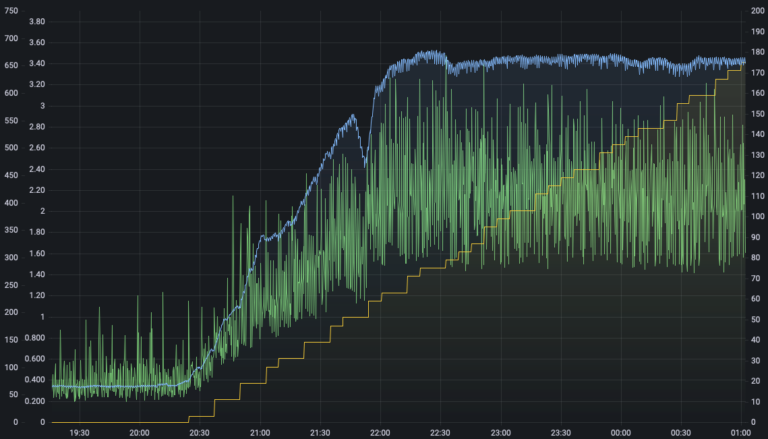
\includegraphics[width=15cm,center]{Figures/cpuValidatorsGossip.png}
    \caption{Graph showing the effect on CPU usage (green line, scale up to 3.80 in GHz) and gossip messages per second (blue line, scale up to 750 messages/sec ), as the number of validators running on one node increases (yellow line, scale up to 200 clients). \cite{Sutton2022ExploringSymphonious}}
    \label{Figure:validatorIncrease}
\end{figure}

An expected linear correlation can be seen between the increasing number of validators and CPU usage, but only up to 60 validators. However, after the 60-70 validator range, the CPU usage and the gossip messages per second level off and seem unaffected by the steadily increasing validators. Other sources that support  this finding - \cite{Roy2022StakingExchange} and \cite{2021HardwareEthstaker}.

Storage space was falsely expected to be a limiting factor as running a single validator takes up almost 2TB of storage. However, after the first validator already has a local copy of the blockchain synced, adding more validators only requires storing a few extra validator keys.

This finding can be explained by understanding Sharding and attestations(\sref{Sharding}). In each epoch (an epoch has 32 slots), 32 randomly selected block proposers propose one block per slot. The remaining validators are not only assigned 1/32 slots that they need to attest the new block for (vote on its validity) but also to possibly one of 64 voting committees. Unaggregated votes from these committees are aggregated and pushed out on specific gossip channels by certain validators assigned to do so. 

Nodes that are not running validators will only subscribe to the gossip topics that push out aggregated votes. But with each validator that you run, they will first need to subscribe to gossip channels with aggregated attestations but occasionally also to gossip topics with unaggregated attestations if they're selected to aggregate the votes for that slot. Hence, up to 64 validators, validators are subscribing and processing more and more gossip messages but past this, there are no new gossip topics to subscribe to and the CPU usage and gossip messages per second level off, as shown in \fref{Figure:validatorIncrease}.

We tried to replicate this behaviour using logarithmic functions and exponential decay functions. Through extended experimentation and applying prior knowledge, we found that the exponential decay function (increasing form), equat{eqn: ExpDecayGeneral} ref{eqn: ExpDecayGeneral}, most accurately matches the characteristics we are looking for because it increases at a slower rate at the beginning and then levels off as more validator clients are added to the node. This is consistent with \ref{Figure:validatorIncrease} that grows almost linearly until 64 validators, after which it levels off. The general equation is:

\begin{equation}
    \label{eqn: ExpDecayGeneral}
    \boldsymbol{\mathrm{E(\mathrm{x})} = \mathrm{A} (1-\mathrm{e}^{-\mathrm{k}(\mathrm{x})}) + \mathrm{C}}
\end{equation}

The lower limit or Y-intercept, $\boldsymbol{\mathrm{C}}$, can be set to the energy measurement obtained for running a single validator client on a specific hardware configuration of a node, denoted by $\boldsymbol{\mathrm{V_{1}}}$. As seen in \fref{Figure:validatorIncrease}, the CPU approaches its maximum capacity as the number of validators approaches 64, after which it levels off. Meanwhile, the SSD is not operating at its maximum capacity. Hence, the asymptotic upper limit of the graph $\boldsymbol{\mathrm{A}}$, can be set to $\boldsymbol{\mathrm{\overline{P}}_{TDP}}$ due to the aforementioned reasoning (\sref{TDPReasoning}). The equation already has its lower limit set to running a single validator, and this equation will only be employed for cases where there are multiple validator clients being run on a single node. Thus, $\boldsymbol{\mathrm{x}}$ denotes the number of additional validator clients run on a node and can only take values from the set of all positive integers.  $\boldsymbol{\mathrm{k}}$, the growth rate constant determines how quickly the energy consumption increases as the validators increase and can be calculated for each node on a case-by-case basis. However, to simplify the equation, we can remove the $\boldsymbol{ + \mathrm{C}}$ as it simply acts as a transition upwards to the graph output by this equation. Removing this transition means we have to subtract $\boldsymbol{ \mathrm{C}}$ from our asymptote $\boldsymbol{\mathrm{\overline{P}}_{TDP}}$. This modification leaves an equation that outputs the extra electricity consumed by $\boldsymbol{\mathrm{x}}$ additional validators:

\begin{equation}
    \label{eqn:ExpDecay}
    \boldsymbol{\mathrm{\overline{V}(\mathrm{x})} = \left(\mathrm{\overline{P}}_{TDP} -\mathrm{\overline{V}_{1}} )\right(1-\mathrm{e}^{-\mathrm{k}(\mathrm{x})}) \qquad \forall x \in \mathbb{Z}^+}
\end{equation}


\begin{figure}[htb!]
    \centering
    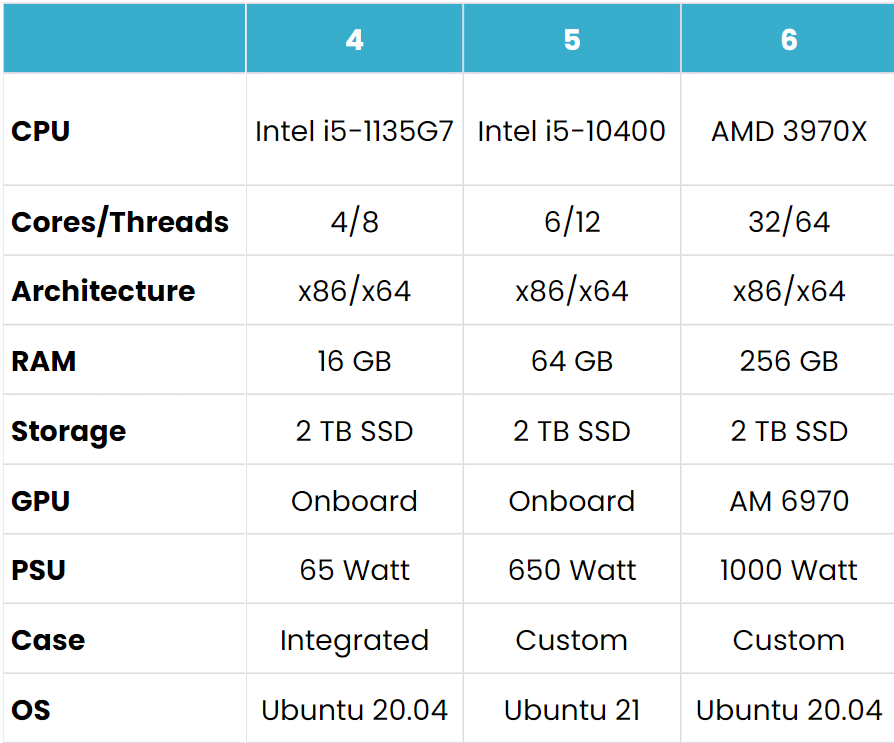
\includegraphics[width=10cm,center]{Figures/CCRIhardwareConfigEdit.png}
    \caption{Table with hardware configurations of a low-tier, mid-tier and high-tier node relative to the hardware recommendation to run a validator node shown in table \ref{Table:RecommendedHardware}. Source: CCRI report \cite{CryptoCarbonRatingsInstitute2022TheNetwork}, table 6. Configurations 1,2, and 3 were omitted due to being unable to run the client software.}
    \label{Figure:CCRIhardwareConfig}
\end{figure}

\label{DetermineK}
Here is an example calculation to determine constant $\boldsymbol{\mathrm{k}}$ for an average node, configuration 6, shown in figure \ref{Figure:CCRIhardwareConfig}. 

$\boldsymbol{\mathrm{C}} = \boldsymbol{\mathrm{150.20}} $ Watts, assuming the node runs the most common CL and EL client combination, Prysm and Geth. Mean values are taken from  \cite{CryptoCarbonRatingsInstitute2022TheNetwork}.

$\boldsymbol{\mathrm{A}} = $ TDP rating for AMD 3970X, $\boldsymbol{\mathrm{280}} $ Watts \cite{AMDDatabase} subtracted by the $\boldsymbol{\mathrm{C}}$ value which results in $\boldsymbol{\mathrm{129.80}}$ W.

We can set $\boldsymbol{\mathrm{x}} $ can be set to $\boldsymbol{\mathrm{63}} $, as the graph starts at 1 validator running already, totalling 64 validators. We assume that the CPU is operating at just 10\% below its maximum capacity (TDP rating) at the 64$^\mathrm{{th}}$ total validator and equate the left side of the equation to $\boldsymbol{\mathrm{0.9 * TDP}} = 252$ W. This needs to be subtracted by $\boldsymbol{\mathrm{C}}$ to account for translating the graph upwards earlier, resulting in $\boldsymbol{\mathrm{252-150.20 = 101.8}}$W. 

\begin{equation*}
    \boldsymbol{\mathrm{129.8} * (1-\mathrm{e}^{-\mathrm{k}(\mathrm{63})}) = \mathrm{101.80}}
\end{equation*}

Which solves to:
\begin{equation*}
    \boldsymbol{\mathrm{k} = \mathrm{{2.435} * {10}^{-2}}}
\end{equation*}

Figure \ref{Figure:MultipleValidators} graphs the example introduced above.

% MultipleValidators graph_________
\begin{figure}[htb!]
    \centering
    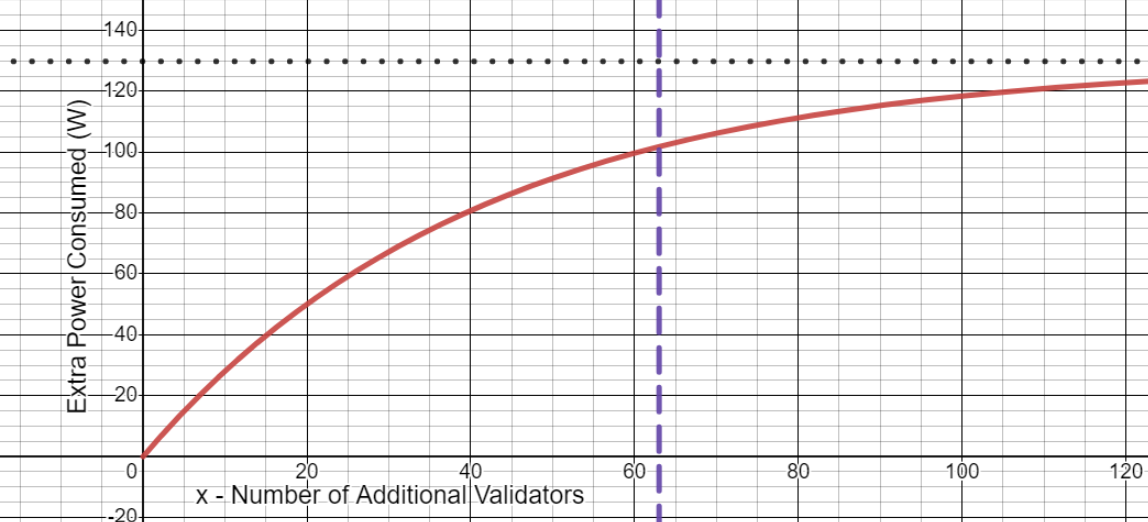
\includegraphics[ width=14cm,center]{Figures/AsymptoteMultipleValidators.png}
    \caption{A plot of \eref{eqn:ExpDecay} showing its inverse exponential decay behaviour for configuration 6 from figure \ref{Figure:CCRIhardwareConfig}. The asymptote at $\boldsymbol{\mathrm{A = 129.80}}$W is highlighted y the horizontal dotted black line. A dashed vertical purple line also highlights the value of the curve to be $\boldsymbol{\mathrm{101.8}}$W at $\boldsymbol{\mathrm{x = 63}}$ which is the 64$^\mathrm{th}$ validator on that node.}
    \label{Figure:MultipleValidators}
\end{figure}

\eref{eqn:ExpDecay} is case specific and can be applied independently to estimate the electricity usage of a node with a specific combination of EL and CL clients as well as a specific hardware combination. To integrate this equation into the one proposed earlier, \eref{eqn:CCRISync}, it will need to be generalised, keeping all combinations of hardware and clients in mind.

$\boldsymbol{\mathrm{\overline{V}_{1}}}$ captures the electricity consumed by a node on average across all hardware configurations and clients that we have data for. 

\begin{equation*}
    \boldsymbol{\mathrm{\overline{V}_{1}} = {\frac{\displaystyle\sum\limits_{i=1}^{n}{ \left({\left(\mathrm{\overline{P}}_{ID} + \mathrm{\overline{P}}_{CL} + \mathrm{\overline{P}}_{EL}\right)} * {\phi_{EL,CL}} \right)}}
{\pi}} }
\end{equation*}

Following this, \eref{eqn:CCRISync} introduced earlier can be re-written as:

\begin{equation*}
     \boldsymbol{\overline{\mathrm{P}}_{SNC} +  \overline{\mathrm{V}}_{1} 
} 
\end{equation*}

When modified to account for $\boldsymbol{\mathrm{x }}$ additional validator clients being run on the same node: 

\begin{equation*}
     \boldsymbol{\mathrm{P}_{SNC} +  \overline{\mathrm{V}}_{1} + \mathrm{\overline{V}(\mathrm{x})}} 
\end{equation*}

Which can be expanded to:
\begin{equation}
    \label{eqn:FinalEqnShort}
     \boldsymbol{\mathrm{P}_{SNC} +  \overline{\mathrm{V}}_{1} + {\left(\mathrm{\overline{P}}_{TDP} -\overline{\mathrm{V}}_{1} )\right(1-\mathrm{e}^{-\mathrm{k}(\mathrm{x})}) \qquad \forall x \in \mathbb{Z}^+}} 
\end{equation}

Expanding all terms results in this final equation:
\begin{align}
\label{eqn:FinalEqnLong}
     &\boldsymbol{({\mathrm{T}_{EL} * ({\mathrm{P}_{TDP}} + \mathrm{P}_{SSD})}) +  {\frac{\displaystyle\sum\limits_{i=1}^{n}{ \left({\left(\mathrm{\overline{P}}_{ID} + \mathrm{\overline{P}}_{CL} + \mathrm{\overline{P}}_{EL}\right)} * {\phi_{EL,CL}} \right)}}
{\pi}}}\nonumber \\  \nonumber\\  
     &\boldsymbol{+ {(\mathrm{\overline{P}}_{TDP} - {\frac{\displaystyle\sum\limits_{i=1}^{n}{ \left({\left(\mathrm{\overline{P}}_{ID} + \mathrm{\overline{P}}_{CL} + \mathrm{\overline{P}}_{EL}\right)} * {\phi_{EL,CL}} \right)}}
{\pi}}} ) (1-\mathrm{e}^{-\mathrm{k}(\mathrm{x})})}\\ \nonumber \\    
     &\boldsymbol{\qquad \qquad \qquad \qquad \qquad \qquad \forall \text{ } x \in \mathbb{Z}^+}\nonumber 
\end{align}

Note that hardware configuration-specific terms, such as TDP and SSD power usage, must be weighted according to the estimated usage of that hardware by all users across the network to generalise the network's cumulative electricity consumption. 

% ___________________________________________________________________MODELS DONE< NOW 

% MODEL AAAAAAAAAAAAAAAAAAAAAAAAAAAAAAAAAAAAAAAAAAAAAAAAAA
\section{Implementing 'Model A'}

\textbf{Average Sync Energy of a node}

First, 3 hardware configurations must be chosen, including a low, medium and high tier for running validator nodes. The recommended hardware configuration for a Geth client ($\sim$ 70\% network share) is shown in \tref{Table:RecommendedHardware}.

\begin{table}[h]
\centering
\begin{tabular}{|l|l|}
\hline
Solo Validator Nodes        & \begin{tabular}[c]{@{}l@{}}Quad Core Processor, \\ 2TB SSD , 16GB memory\end{tabular}                            \\ \hline
Archive Nodes               & \begin{tabular}[c]{@{}l@{}}Quad Core or Dual Core Hyperthreaded \\ Processor, 12TB SSD, 16GB memory\end{tabular} \\ \hline
Minimum for Validator nodes & \begin{tabular}[c]{@{}l@{}}Dual Core Hyperthreaded, \\ 1TB SSD, 4GB memory\end{tabular}                          \\ \hline
\end{tabular}
\caption{Recommended hardware configurations for running various nodes by Geth \cite{2022DeveloperGo-ethereum}}
\label{Table:RecommendedHardware}
\end{table}

A combination of hardware that closely matches the recommendation by Geth developers must be chosen to fulfil the aim of PoS Ethereum nodes being run on commodity hardware. Performing such data collection is out of the scope of this report. Due to the limited availability of empirical data on hardware running Ethereum after 'the Merge', the hardware configurations 4,5 and 6 in \fref{Figure:CCRIhardwareConfig} from the CCRI report \cite{CryptoCarbonRatingsInstitute2022TheNetwork} are used. Using this data also helps draw fairer comparisons when evaluating Model A later on. 

Synchronising energy: 
For the first part of \eref{eqn:FinalEqnShort} denoted by $\boldsymbol{\mathrm{P}_{SNC}}$, no empirical data was available in the CCRI report about this synchronisation stage. Non-scientific data for synchronisation time $\boldsymbol{\mathrm{T}_{EL}}$ for users employing varying combinations of hardware and EL clients can be found in \tref{Table:ELRunTime} of the appendix. This limited data is insufficient to differentiate between the sync times for all 4 clients but allows us to roughly estimate the average sync time on varying hardware configurations (relative to \fref{Figure:CCRIhardwareConfig})  in \tref{Table:SyncEnergy}. Geth was given a higher weighting in this estimation as used by  $\sim$ 70\% of the network. 

Varying user needs affect their decision in choosing hardware, ranging from different profit structures to low-budget devices and future-proof hardware. There is an immeasurable amount of hardware configurations that users could opt for. Thus, we model this distribution of users between the 3 categories of hardware using a continuous distribution, particularly - the CDF (Cumulative distribution function) of the standard normal distribution. The distribution was divided into 3 parts, 25\% of the network assumed to opt for the low-tier hardware (configuration 4), 50\% for the mid-tier (configuration 5) and 25\% for the high-tier (configuration 6). 

\begin{table}[h]
\centering
\begin{tabular}{|l|l|l|l|l|}
\hline
\textbf{Tier} & \textbf{$\boldsymbol{\mathrm{T}_{EL}}$ {[}h{]}} & \textbf{$\boldsymbol{\mathrm{P}_{TDP}}$ {[}Wh{]}} & \textbf{$\boldsymbol{\mathrm{P}_{SSD}}$ {[}Wh{]}} & \textbf{Share of the network {[}\%{]}} \\ \hline
Low    & 36 & 28  & 3.5 & 25 \\ \hline
Medium & 24 & 65  & 8.5 & 50 \\ \hline
High   & 12 & 280 & 10  & 25 \\ \hline
\end{tabular}
\caption{The estimated synchronisation times for varying tiers of hardware configurations relative to \fref{Figure:CCRIhardwareConfig} and their estimated share of the network. Sources for $\boldsymbol{\mathrm{P}_{TDP}}$ : \cite{IntelFAQs}, \cite{AMDDatabase}. Source for $\boldsymbol{\mathrm{P}_{SSD}}$: \cite{RachanaKhamamkar2020AnalyzingDrives}}
\label{Table:SyncEnergy}
\end{table}

The split of the share of the network estimated for each hardware tier in \tref{Table:SyncEnergy} is similar to the CCRI report \cite{CryptoCarbonRatingsInstitute2022TheNetwork} to allow for fair comparisons later on. 

Given this data, the $\boldsymbol{\mathrm{P}_{SNC}}$ for an average node can be calculated by following its formula with each hardware tier multiplied by its network share: \newline
\begin{align}
    &\boldsymbol{0.25*(36*(28 + 3.5)) + 0.5*(24*(65+8.5)) + 0.25*(12*(280+10))} \nonumber\\ \nonumber \\
    &\boldsymbol{{\mathrm{P}_{SNC}} = 2035.5} \text{ Wh} \nonumber
\end{align}


% ________________________________________--

% _---------------------------------------
\textbf{Average electricity consumption of a node after synchronisation}
\label{postSyncEnergyImplementation}
For the next part of \eref{eqn:FinalEqnShort}, $\boldsymbol{\mathrm{\overline{V}_{1}}}$ needs to be calculated. First, the \tref{Table:ClientShares} shows the updated values for EL and CL clients' shares of the Ethereum network that will be used to calculate $\boldsymbol{\phi_{EL,CL}}$.  

% --------------------------------------
\begin{table}[h]
    \centering

  \subcaptionbox{\textbf{Execution Clients} \cite{Sigp/blockprint:Metrics}}{
      \begin{tabular}{|l|c|}
            \hline
             Geth & 69.22 \% \\
            \hline
             Nethermind & 14.16 \%  \\
            \hline 
             Erigon & 10.65 \% \\
            \hline
             Besu & 5.78 \% \\
            \hline
             OpenEthereum & 0.00 \% \\
            \hline
             Other & 0.20 \% \\
            \hline
  \end{tabular}
    \label{Table:ClientShares:left}
  }
  \subcaptionbox{\textbf{Consensus Clients}  \cite{ClientsExplorer}}{
        \begin{tabular}{|l|c|}
                    \hline
             Prysm & 65.15 \%  \\
            \hline
             Lighthouse & 29.30 \% \\
            \hline 
             Teku & 10.65 \% \\
            \hline
             Nimbus & 0.91 \% \\
            \hline
             Lodestar & 0.0 \% \\
            \hline
             Other & 0.0 \%  \\
            \hline
            
  \end{tabular}
    \label{Table:ClientShares:right}
  }
    \caption{An updated table of client diversity within Ethereum Mainnet network, data recorded on 27-Mar 23. Updates table 5 from report \cite{CryptoCarbonRatingsInstitute2022TheNetwork} }
  \label{Table:ClientShares}
\end{table}

% --------------------------------------------

Ever since the CCRI report, OpenEthereum has been deprecated, and Lodestar no longer holds a sizeable share of the network, and they were not included in calculations.  

Empirical data on the mean consumption values recorded for all 3 hardware configurations running all clients were collected in \tref{Table:ConsumptionValues}, taken from the CCRI report \cite{CryptoCarbonRatingsInstitute2022TheNetwork}. The Nethermind client which now holds a sizeable share of the network, has no empirical electricity consumption data available. To estimate this, the other 3 EL clients' values were averaged for each configuration.

% ----------------------
\begin{table}[htb!]
\centering
\begin{tabular}{|l|lll|}
\hline
\textbf{Client Name} & \multicolumn{3}{l|}{\textbf{Node Configuration}}                               \\ \hline
\textbf{}            & \multicolumn{1}{l|}{\textbf{4}} & \multicolumn{1}{l|}{\textbf{5}} & \textbf{6} \\ \hline
Idle Node                & \multicolumn{1}{l|}{3.66}       & \multicolumn{1}{l|}{25.04}      & 78.17      \\ \cline{1-1}
Geth (EL)            & \multicolumn{1}{l|}{11.23}      & \multicolumn{1}{l|}{9.70}       & 47.70      \\ \cline{1-1}
Erigon (EL)          & \multicolumn{1}{l|}{18.60}      & \multicolumn{1}{l|}{17.59}      & 44.62      \\ \cline{1-1}
Besu (EL)            & \multicolumn{1}{l|}{30.25}      & \multicolumn{1}{l|}{31.02}      & 75.04      \\ \cline{1-1}
Nethermind(EL)[Averaged] & \multicolumn{1}{l|}{20.03}       & \multicolumn{1}{l|}{19.44}       & 55.79      \\ \cline{1-1}
Prysm (CL)           & \multicolumn{1}{l|}{3.51}       & \multicolumn{1}{l|}{2.87}       & 24.33      \\ \cline{1-1}
Lighthouse (CL)      & \multicolumn{1}{l|}{2.75}       & \multicolumn{1}{l|}{3.14}       & 18.84      \\ \cline{1-1}
Teku (CL)            & \multicolumn{1}{l|}{3.71}       & \multicolumn{1}{l|}{3.32}       & 27.46      \\ \cline{1-1}
Nimbus (CL)          & \multicolumn{1}{l|}{1.67}       & \multicolumn{1}{l|}{2.08}       & 17.11      \\ \cline{1-1}
Lodestar(CL)         & \multicolumn{1}{l|}{3.14}       & \multicolumn{1}{l|}{3.89}       & 33.55      \\ \hline

\end{tabular}
\caption{Mean electricity consumption values in Watts, measured in the report \cite{CryptoCarbonRatingsInstitute2022TheNetwork} for nodes with configurations 4-6 mentioned in  \fref{Figure:CCRIhardwareConfig} running various clients.  }
\label{Table:ConsumptionValues}
\end{table}

Given this data, we are able to calculate the values in \tref{Table:EstimatesPerNode}. As an example, the first row (Prysm,Geth) was calculated by adding each electricity usage when idle, running Pyrsm, and running Geth multiplied by the share of the hardware tier, for each configuration.
\begin{align}
    &\boldsymbol{0.25*(3.66 + 11.23 + 3.51) + 0.50 * (25.04 + 9.70 + 2.87) + 0.25} \nonumber\\
    &\boldsymbol{* (78.17 + 47.70 + 24.33) = 69.96}\text{Wh} \nonumber
\end{align}

% -----------------------------------------
\begin{table}[htb!]
\centering
\begin{tabular}{|ll|l|l|l|}
\hline
\multicolumn{2}{|l|}{\textbf{Client Combination}} &
  \multirow{2}{*}{\textbf{\begin{tabular}[c]{@{}l@{}}Estimate\\ {[}Wh{]}\end{tabular}}} &
  \multirow{2}{*}{\textbf{\begin{tabular}[c]{@{}l@{}}Annualised Estimate\\ {[}kWh/year{]}\end{tabular}}} &
  \multirow{2}{*}{\textbf{\begin{tabular}[c]{@{}l@{}}Client Combination\\ Share {[}\%{]}\end{tabular}}} \\ \cline{1-2}
\multicolumn{1}{|l|}{\textbf{CL Client}} & \textbf{EL Client} &       &        &       \\ \hline
\multicolumn{1}{|l|}{Prysm}              & Geth               & 60.96 & 533.97 & 45.10 \\ \cline{1-2}
\multicolumn{1}{|l|}{Prysm}              & Erigon             & 65.97 & 577.91 & 6.94  \\ \cline{1-2}
\multicolumn{1}{|l|}{Prysm}              & Besu               & 83.21 & 728.88 & 3.77  \\ \cline{1-2}
\multicolumn{1}{|l|}{Prysm}              & Nethermind         & 70.05 & 613.62 & 9.23  \\ \cline{1-2}
\multicolumn{1}{|l|}{Lighthouse}         & Geth               & 59.53 & 521.47 & 20.28 \\ \cline{1-2}
\multicolumn{1}{|l|}{Lighthouse}         & Erigon             & 64.54 & 565.41 & 3.12  \\ \cline{1-2}
\multicolumn{1}{|l|}{Lighthouse}         & Besu               & 81.78 & 716.38 & 1.69  \\ \cline{1-2}
\multicolumn{1}{|l|}{Lighthouse}         & Nethermind         & 68.62 & 601.11 & 4.15  \\ \cline{1-2}
\multicolumn{1}{|l|}{Teku}               & Geth               & 62.01 & 543.24 & 7.37  \\ \cline{1-2}
\multicolumn{1}{|l|}{Teku}               & Erigon             & 67.03 & 587.18 & 1.13  \\ \cline{1-2}
\multicolumn{1}{|l|}{Teku}               & Besu               & 84.26 & 738.15 & 0.62  \\ \cline{1-2}
\multicolumn{1}{|l|}{Teku}               & Nethermind         & 71.11 & 622.88 & 1.51  \\ \cline{1-2}
\multicolumn{1}{|l|}{Nimbus}             & Geth               & 58.29 & 510.66 & 0.63  \\ \cline{1-2}
\multicolumn{1}{|l|}{Nimbus}             & Erigon             & 63.31 & 554.59 & 0.10  \\ \cline{1-2}
\multicolumn{1}{|l|}{Nimbus}             & Besu               & 80.54 & 705.57 & 0.05  \\ \cline{1-2}
\multicolumn{1}{|l|}{Nimbus}             & Nethermind         & 67.39 & 590.31 & 0.13  \\ \hline
\end{tabular}
\caption{Electricity consumption estimates per node for all possible client combinations along with corresponding annualised values and each client combination's network share. Individual client shares found in \tref{Table:ClientShares}  }
\label{Table:EstimatesPerNode}
\end{table}

% -----------------------------------
$(60.96*45.1) + 65.97*6.94 + 83.21*3.77 + 70.05*9.23 + 59.53*20.28 + 64.54*3.12 + 81.78*1.69 + 68.62*4.15 + 62.01 * 7.37 + 67.03*1.13 + 84.26*0.62 + 71.11 * 1.51 + 58.29*0.63 + 63.31*0.1 + 80.54*0.05 + 67.39*0.13 / 105.82$
Best guess for an individual node: \textbf{63.7613088 Wh}
Annualised value for an individual node assuming 8760h in a year: \textbf{558.549065318 kWh/year}

Assuming the node needs to perform a fresh synchronisation once a year, the annual total consumption of an average node (running 1 validator each) $ \boldsymbol{ \mathrm{\overline{V}_{1}} + \mathrm{P}_{SNC} =}$ \textbf{560.584565318 kWh/year} or \textbf{63.99 Wh}.

Data as of 10$\mathrm{^{th}}$ April 23: \\
Number of nodes connected to Ethereum mainnet: \textbf{12242 nodes} \cite{NodewatchAnalytics} \\
Number of transactions completed each day: \textbf{1074596 tx/day}  \cite{EthereumBlockchair} \\
Number of validators on the network: \textbf{562729 validators} \cite{EthereumEthereum.orgc}


My model: \\
Hourly electricity consumption of the network (running 1 validator each): \textbf{783.37 kWh} \\
Annual electricity consumption of the network (running 1 validator each): \textbf{6.86 GWh} \\
Annual electricity consumption of a single node (running 1 validator each) per transaction: \textbf{0.001429 Wh/tx} \\
Annual electricity consumption of the network (running 1 validator each) per transaction: \textbf{17.50 Wh/tx} \\

CCRI model: \\
Annual electricity consumption of the network (running 1 validator each): \textbf{6.84 GWh} \\
Annual electricity consumption of a single node (running 1 validator each) per transaction: \textbf{0.001424 Wh/tx} \\
Annual electricity consumption of the network (running 1 validator each) per transaction: \textbf{17.43 Wh/tx} \\

% --------------------------------------------------
% STAGE 3 of implementation with multiple validators
% --------------------------------------------------
\textbf{Additional consumption from some nodes running multiple validators}

To include the fact that some nodes are running multiple validators, we implement the final part of \eref{eqn:FinalEqnShort}, calculating the $\boldsymbol{\mathrm{\overline{V}(\mathrm{x})}}$. 

We know from \sref{AdditonalNodesReasoning} that mid-tier nodes can run upto 1000 nodes while high-tier nodes can run 2500+ nodes \cite{2021HardwareEthstaker} \cite{Kaushal2022ValidatingConference}. To use the exponential decrease in electricity consumption to their advantage, when users run additional validator nodes, they often run a minimum of 1000+. Since there are 561,472 validators, we assume that 1000+ additional validators are run by $\sim$562 nodes, using mid to high-tier hardware.   

$\boldsymbol{\mathrm{\overline{P}}_{TDP}}$ can be calculated from \tref{Table:SyncEnergy}: \textbf{205 Wh} \\
$\boldsymbol{ \overline{\mathrm{V}}_{1}}$ calculated in \sref{postSyncEnergyImplementation} : \textbf{63.99 Wh} 

$\boldsymbol{\mathrm{k}}$ can be calculated by the method shown in \sref{DetermineK}:

\begin{equation*}
    \boldsymbol{\mathrm{141.01} * (1-\mathrm{e}^{-\mathrm{k}(\mathrm{63})}) = \mathrm{120.51}}
\end{equation*}

Which solves to:
\begin{equation*}
    \boldsymbol{\mathrm{k} = \mathrm{{3.06096} * {10}^{-2}}}
\end{equation*}

Finally, $\boldsymbol{\mathrm{x}}$ can be set to \textbf{1000} additional validators for 562 of the total nodes on the network while the rest run no additional nodes.

Following the formula, we get $\boldsymbol{\mathrm{\overline{V}(\mathrm{1000})}} =$ \textbf{141.1 Wh}

The hourly consumption of the network will rise by $141.1 * 562 = $ \textbf{79.298 kWh}

The new hourly consumption of the entire network: \textbf{862.66378 kWh} 

The final results can be found in \tref{Table:FinalResults}.
% The new hourly electricity consumption of a single node can be derived: \textbf{70.47} Wh
% Annual electricity consumption of a single node: 617.30 kWh 
% Annual electricity consumption of the network: 7.5569 GWh
% Annual electricity consumption of a single node per transaction: 0.0015738 Wh/tx
% Annual electricity consumption of the network per transaction: 19.27 Wh/tx


% ____________________________________________________________________________
\subsection{Assumptions}

\begin{itemize}
    \item They have taken the syncing on nodes into account into their model whereas for general modelling, it would be  abetter estimate to ignore this initial set up energy and get an avergae form then on. That is what this paper has done, taking averages of the Raspberry Pi rather than including the syncing energy.
    \item The TDP + SSD power usage can be used as an upper limit for the electricity consumption of any hardware set-up
    \item That growth for more than one validator can be modelled by an exponential decay (increasing form)
    \item This exponential growth has an upper limit of TDP + SSD power usage and using the single validator energy consumption as the lower limit
    \item Equation from CCRI gives an accurate estimation and is a good base for my equation
    \item The EL and CL clients are not changed; just additional Validator clients are run on the same set up
    \item 10\% lower than the TDP power should be reached by the time the 64$^\mathrm{{th}}$ validator is run.
    \item Took averages of other EL layer clients per confirguration for NetherMind. not good.
    \item All these numbers are for running a full node, not validators which sdmieler,2020 said is basically negligible
    \item high, mid low tiers dont have a fair distribution of hardware but does help achieve more accurate results hopefully
    \item for table \_\_ gave higher importance to Geth to estimate sync time as it has a much larger share of the network than the other EL clients
\end{itemize}

\section{Implementing other models}

As mentioned in \sref{LitRevExistingModels} there are two existing models found in the wider literature. 

\textbf{The 'CCRI' model} 

As discussed in \sref{CCRIBaseEqnSection} before, this model from report \cite{CryptoCarbonRatingsInstitute2022TheNetwork}, forms the $ \boldsymbol{\overline{\mathrm{V}}_{1}}$ part of Model A from this report. Thus, all the data gathering and calculations have already been performed in \sref{postSyncEnergyImplementation}. Updated values from \tref{Table:ClientShares} and \tref{Table:ConsumptionValues} were used to populate \tref{Table:EstimatesPerNode}. The split in network share between the 3 hardware tiers (low, mid and high-tier) was done binomially rather than a continous distribution. However, the split percentages remain the same (25\%, 50\%, 25\% respectively), making the results more comparable. Final results for this model can be found in \tref{Table:FinalResults}.

\textbf{The 'UCL' model} 

The original version of this UCL model can be found in report \cite{Platt2022TheProof-of-Work}. However, the authors of that report released an updated report \cite{IbanezTheExpansion}, last revised on 7$\mathrm{^{th}}$ Feb 23. Because this report is so recent, data from its Results section can be directly taken and updated with the latest node count and transaction amounts used to implement Model A in this report (\sref{postSyncEnergyImplementation}). Resulting values can be found in \tref{Table:FinalResults}. 





% ______________________________________________________________________
% \section {Modelling Ethereum's Carbon Emissions}
% \url{https://ethernodes.org/countries}

% \paragraph{ Simple Linear Regression Model}
% A simple logical model for estimating the energy consumption of Ethereum 2.0's energy consumption logically would be using simple regression. y = mx + c, and if we wanted to say that energy is dependent on transactions, then we can say y is the energy per node, m is the slope we need to find, x is the number of transactions/sec, c is the base energy an idle node requires. Then we multiply this whole thing by the number of validators on the network to get the overall network energy consumption.

% ____________________________________________________________________________
\section{Discussion and Evaluation Of Models}
% ____________________________________________________________________________
\subsection{Final Results}



% -----------------------------------------------
% RESULTS  TABLEEEE
% ----------------------------------------------------------------
\begin{table}[h]
\begin{tabular}{ll"ll"l"l|}
\cline{3-6}
 &
   &
  \multicolumn{2}{l"}{\textbf{Model A}} &
  \textbf{CCRI \cite{CryptoCarbonRatingsInstitute2022TheNetwork}} &
  \textbf{UCL \cite{IbanezTheExpansion}} \\ \thickhline
\multicolumn{1}{|l|}{\multirow{2}{*}{\textbf{\begin{tabular}[c]{@{}l@{}}Accounts \\ For:\end{tabular}}}} &
  \textbf{\begin{tabular}[c]{@{}l@{}}Synchronisation \\ Energy \end{tabular}} &
  \multicolumn{1}{l|}{Yes} &
  Yes &
  No &
  No \\ \cline{2-6} 
\multicolumn{1}{|l|}{} &
  \textbf{\begin{tabular}[c]{@{}l@{}}Additional Validators \\ Per Node\end{tabular}} &
  \multicolumn{1}{l|}{No} &
  Yes &
  No &
  No \\ \hline
\multicolumn{1}{|l|}{\multirow{2}{*}{\textbf{Hourly}}} &
  \textbf{\begin{tabular}[c]{@{}l@{}}Per Node \\ {[}Wh{]}\end{tabular}} &
  \multicolumn{1}{l|}{63.99} &
  70.47 &
  63.76 &
  85.03 \\ \cline{2-6} 
\multicolumn{1}{|l|}{} &
  \textbf{\begin{tabular}[c]{@{}l@{}}Entire Network \\ {[}kWh{]}\end{tabular}} &
  \multicolumn{1}{l|}{783.37} &
  862.66 &
  780.57 &
  1040.09 \\ \hline
\multicolumn{1}{|l|}{\multirow{4}{*}{\textbf{Annual}}} &
  \textbf{\begin{tabular}[c]{@{}l@{}}Per Node \\ {[}kWh{]}\end{tabular}} &
  \multicolumn{1}{l|}{560.58} &
  617.30 &
  558.55 &
  744.86 \\ \cline{2-6} 
\multicolumn{1}{|l|}{} &
  \textbf{\begin{tabular}[c]{@{}l@{}}Entire Network \\ {[}GWh{]}\end{tabular}} &
  \multicolumn{1}{l|}{6.86} &
  7.56 &
  6.84 &
  9.12 \\ \cline{2-6} 
\multicolumn{1}{|l|}{} &
  \textbf{\begin{tabular}[c]{@{}l@{}}Per Node / Transaction \\ {[}mWh/tx{]}\end{tabular}} &
  \multicolumn{1}{l|}{1.43} &
  1.57 &
  1.42 &
  1.90 \\ \cline{2-6} 
\multicolumn{1}{|l|}{} &
  \textbf{\begin{tabular}[c]{@{}l@{}}Entire Network / Transaction \\ {[}Wh/tx{]}\end{tabular}} &
  \multicolumn{1}{l|}{17.50} &
  19.27 &
  17.43 &
  23.25 \\ \hline
\end{tabular}
\caption{The results (best guess values) obtained from implementing 'Model A' as well as 2 other models, all using the same metrics in \sref{postSyncEnergyImplementation}.}
\label{Table:FinalResults}
\end{table}
After the table comes:
\begin{figure}[!htb]
    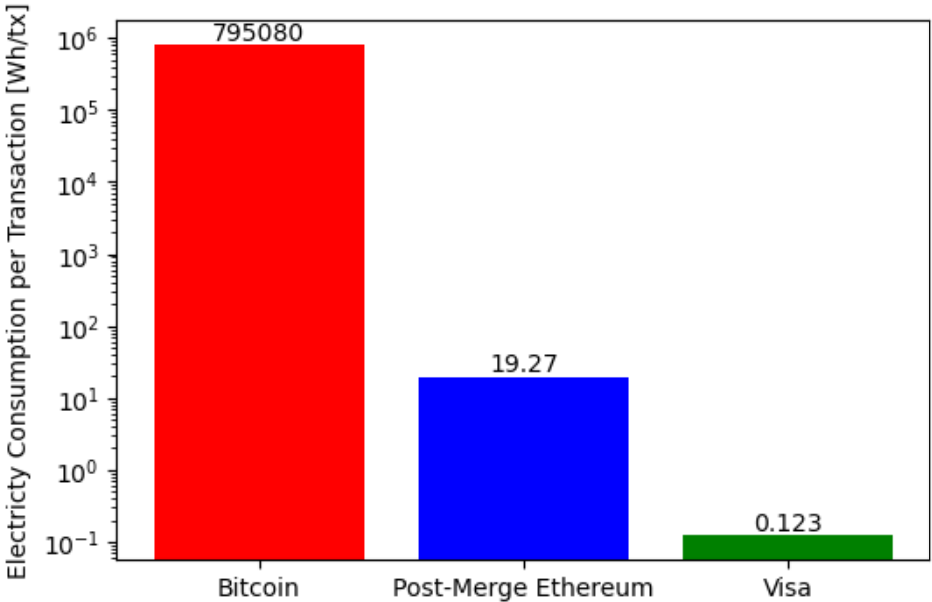
\includegraphics[width=13cm,center]{Figures/ElectricityConsumptionPlot.png}
    \caption{Energy consumption per transaction for Bitcoin \cite{BitcoinDigiconomist}, Ethereum 2.0 [from Model A] and Visa \cite{2022VisaReport}, \cite{VisaHome} plotted on a logarithmic scale. The code is in Appendix C, \fref{Figure:ElectrictyConsumptionPlotCode}}
    \label{Figure:ElectricityConsumptionPlot}
\end{figure}
% ____________________________________________________________________________
\subsection{Interpretation}


% ____________________________________________________________________________
\subsection{Verification and Evaluation}

To verify Model A, other models found in the wider literature have been implemented using updated metrics. The results of my model should lie reasonably close to other models and any discrepencies must be explained. 


% ____________________________________________________________________________
\subsection{Discussion}
*So I did it this way, could've been done another way. My method could've affected the results
* self-reflection -> smaller factors not considered, maybe if I used a different group of numbers/users some other result would have been achieved, loopholes

All data comes from CCRI, couldn't have done such as accurate experiment myself.

Also all electricity values are from software within the computers. Hence are not 'at-wall' values which would really show how much electricity is being drawn from the national grid. Perhaps someone well versed in electrical engineering may be able to add some factor to the overall equation that adjusts for the dissipated energy and gets a more accurate estimation 'At-wall'.

Couldn't use API - may have affected the accuracy of data, could've been live data, more precise data

% __________________________________________________________________________



\section{Future Work}

***API wasnt ready, when it is, data0driven modelling could be pursued.

\section{Critical Evaluation}

\subsection{Project Management Evaluation}

Many different approaches to modelling were tried during the course of the project. Some include sensitivity analysis to check which parameters affect the overall electricity consumption the most when using the PoS consensus protocol \cite{MarionAnModelling}. Some data-driven modelling techniques explored included time series analysis and logistic regression \cite{IbanezTheExpansion} however, the 'The Merge' is a very recent event, and it was hard to obtain any meaningful data on it.  ***talk about the risk table

The original plan of this project was to develop blockchain-based solutions for modelling drug supply chains, but it underwent multiple revisions. This was among the foreseen risks in opting for a blockchain-related topic as it is a relatively new technology. This risk was mitigated by following the pre-planned risk mitigation strategy found in in /ref**** in the appendix.

I learnt that it is simple to understand a simplified model of a complex system; however, to be the one modelling it requires absolute subject-matter expertise. Deep knowledge of cryptocurrencies as well as the Ethereum protocol specifically, had to be acquired in order to expand to the pre-existing models meaningfully. 

\section{Key Points Covered}
